\documentclass[a4paper,11pt]{book}
%\documentclass[a4paper,twoside,11pt,titlepage]{book}
\usepackage{listings}
\usepackage[utf8]{inputenc}
\usepackage[spanish]{babel}

% \usepackage[style=list, number=none]{glossary} %
%\usepackage{titlesec}
%\usepackage{pailatino}

\decimalpoint
\usepackage{dcolumn}
\newcolumntype{.}{D{.}{\esperiod}{-1}}
\makeatletter
\addto\shorthandsspanish{\let\esperiod\es@period@code}
\makeatother


%\usepackage[chapter]{algorithm}
\RequirePackage{verbatim}
%\RequirePackage[Glenn]{fncychap}
\usepackage{fancyhdr}
\usepackage{graphicx}
\usepackage{afterpage}
\usepackage{amsmath}
\usepackage{amsfonts}

\usepackage{float}
\usepackage{longtable}

\usepackage[pdfborder={000}]{hyperref} %referencia
\usepackage{epigraph}
 \setlength{\epigraphwidth}{5in}
 
 
% ******************************************************************** 
% Custom commands Rafael Nogales
% ******************************************************************** 
\DeclareMathOperator{\EX}{\mathbb{E}}% expected value
\DeclareMathOperator{\R}{\mathbb{R}}
\DeclareMathOperator{\sumn}{\sum_{i=1}^n}


% ********************************************************************
% Re-usable information
% ********************************************************************
\newcommand{\myTitle}{Análisis de los algoritmos de Boosting en entornos con ruido de clase.\xspace}
\newcommand{\myDegree}{Doble Grado en Ingeniería Informática y Matemáticas\xspace}
\newcommand{\myName}{Rafael Nogales Vaquero \xspace}
\newcommand{\myProf}{Francisco Herrera Triguero  \xspace}
\newcommand{\myOtherProf}{Salvador García López \xspace}
%\newcommand{\mySupervisor}{Put name here\xspace}
\newcommand{\myFaculty}{Escuela Técnica Superior de Ingenierías Informática y de
Telecomunicación\xspace}
\newcommand{\myFacultyShort}{E.T.S. de Ingenierías Informática y de
Telecomunicación\xspace}
\newcommand{\myDepartment}{Departamento de ...\xspace}
\newcommand{\myUni}{\protect{Universidad de Granada}\xspace}
\newcommand{\myLocation}{Granada\xspace}
\newcommand{\myTime}{\today\xspace}
\newcommand{\myVersion}{Version 0.1\xspace}


\hypersetup{
pdfauthor = {\myName (email (en) ugr (punto) es)},
pdftitle = {\myTitle},
pdfsubject = {},
pdfkeywords = {palabra_clave1, palabra_clave2, palabra_clave3, ...},
pdfcreator = {LaTeX con el paquete ....},
pdfproducer = {pdflatex}
}

%\hyphenation{}


%\usepackage{doxygen/doxygen}
%\usepackage{pdfpages}
\usepackage{url}
\usepackage{colortbl,longtable}
\usepackage[stable]{footmisc}
%\usepackage{index}
\usepackage{algpseudocode}

%\makeindex
%\usepackage[style=long, cols=2,border=plain,toc=true,number=none]{glossary}
% \makeglossary

% Definición de comandos que me son tiles:
%\renewcommand{\indexname}{Índice alfabético}
%\renewcommand{\glossaryname}{Glosario}

\pagestyle{fancy}
\fancyhf{}
\fancyhead[LO]{\leftmark}
\fancyhead[RE]{\rightmark}
\fancyhead[RO,LE]{\textbf{\thepage}}
\renewcommand{\chaptermark}[1]{\markboth{\textbf{#1}}{}}
\renewcommand{\sectionmark}[1]{\markright{\textbf{\thesection. #1}}}

\setlength{\headheight}{1.5\headheight}

\newcommand{\HRule}{\rule{\linewidth}{0.5mm}}
%Definimos los tipos teorema, ejemplo y definición podremos usar estos tipos
%simplemente poniendo \begin{teorema} \end{teorema} ...
\newtheorem{teorema}{Teorema}[chapter]
\newtheorem{ejemplo}{Ejemplo}[chapter]
\newtheorem{definicion}{Definición}[chapter]

\definecolor{gray97}{gray}{.97}
\definecolor{gray75}{gray}{.75}
\definecolor{gray45}{gray}{.45}
\definecolor{gray30}{gray}{.94}

\DeclareMathOperator*{\argmin}{arg\,min} % thin space, limits underneath in displays

 
% minimizar fragmentado de listados
\lstnewenvironment{listing}[1][]
   {\lstset{#1}\pagebreak[0]}{\pagebreak[0]}

\lstdefinestyle{CodigoC}
   {
	basicstyle=\scriptsize,
	frame=single,
	language=C,
	numbers=left
   }
\lstdefinestyle{CodigoC++}
   {
	basicstyle=\small,
	frame=single,
	backgroundcolor=\color{gray30},
	language=C++,
	numbers=left
   }

 
\lstdefinestyle{Consola}
   {basicstyle=\scriptsize\bf\ttfamily,
    backgroundcolor=\color{gray30},
    frame=single,
    numbers=none
   }


\newcommand{\bigrule}{\titlerule[0.5mm]}


%Para conseguir que en las páginas en blanco no ponga cabecerass
\makeatletter
\def\clearpage{%
  \ifvmode
    \ifnum \@dbltopnum =\m@ne
      \ifdim \pagetotal <\topskip
        \hbox{}
      \fi
    \fi
  \fi
  \newpage
  \thispagestyle{empty}
  \write\m@ne{}
  \vbox{}
  \penalty -\@Mi
}
\makeatother

\usepackage{pdfpages}



\begin{document}
\begin{titlepage}
 
 
\newlength{\centeroffset}
\setlength{\centeroffset}{-0.5\oddsidemargin}
\addtolength{\centeroffset}{0.5\evensidemargin}
\thispagestyle{empty}

\noindent\hspace*{\centeroffset}\begin{minipage}{\textwidth}

\centering

\includegraphics[width=0.9\textwidth]{imagenes/logo_ugr.jpg}\\[1.4cm]

\textsc{ \Large TRABAJO FIN DE GRADO\\[0.2cm]}
\textsc{ DOBLE GRADO EN INGENIERÍA INFORMÁTICA Y MATEMÁTICAS }\\[1cm]
% Upper part of the page
% 
% Title
{\Huge\bfseries Análisis de los algoritmos de Boosting en entornos con ruido de clase.\\
}
\noindent\rule[-1ex]{\textwidth}{3pt}\\[3.5ex]
{\large\bfseries Rafael Nogales Vaquero}
\end{minipage}

\vspace{2.5cm}
\noindent\hspace*{\centeroffset}\begin{minipage}{\textwidth}
\centering

\textbf{Autor}\\ {Rafael Nogales Vaquero}\\[2.5ex]
\textbf{Directores}\\
{Francisco Herrera Triguero \\
Julián Luengo Martín}\\[2cm]

\includegraphics[width=0.3\textwidth]{imagenes/etsiit_logo.png}\\[0.1cm]
\textsc{Escuela Técnica Superior de Ingenierías Informática y de Telecomunicación}\\
\textsc{---}\\
Granada, 7 Septiembre de 2018
\end{minipage}
%\addtolength{\textwidth}{\centeroffset}
%\vspace{\stretch{2}}
\end{titlepage}



\chapter*{}
%\thispagestyle{empty}
%\cleardoublepage

%\thispagestyle{empty}

\begin{titlepage}
 
 
\setlength{\centeroffset}{-0.5\oddsidemargin}
\addtolength{\centeroffset}{0.5\evensidemargin}
\thispagestyle{empty}

\noindent\hspace*{\centeroffset}\begin{minipage}{\textwidth}

\centering
%
\includegraphics[width=0.9\textwidth]{imagenes/logo_ugr.jpg}\\[1.4cm]

%\textsc{ \Large PROYECTO FIN DE CARRERA\\[0.2cm]}
%\textsc{ INGENIERÍA EN INFORMÁTICA}\\[1cm]
% Upper part of the page
% 

 \vspace{3.3cm}

%si el proyecto tiene logo poner aquí
%
\includegraphics{imagenes/logo.png} 
% \vspace{0.5cm}

% Title

{\Huge\bfseries Análisis de los algoritmos de Boosting en entornos con ruido de clase.\\
}
\noindent\rule[-1ex]{\textwidth}{3pt}\\[3.5ex]
%{\large\bfseries .\\[4cm]}
\end{minipage}

\vspace{2.5cm}
\noindent\hspace*{\centeroffset}\begin{minipage}{\textwidth}
\centering

\textbf{Autor}\\ {Rafael Nogales Vaquero}\\[2.5ex]
\textbf{Directores}\\
{Francisco Herrera Triguero\\
Julian Luengo Martín}\\[2cm]
%
\includegraphics[width=0.15\textwidth]{imagenes/tstc.png}\\[0.1cm]
%\textsc{Departamento de Teoría de la Señal, Telemática y Comunicaciones}\\
%\textsc{---}\\
%Granada, mes de 201
\end{minipage}
%\addtolength{\textwidth}{\centeroffset}
\vspace{\stretch{2}}

 
\end{titlepage}






\cleardoublepage
\thispagestyle{empty}

\begin{center}
{\large\bfseries Análisis de los algoritmos de Boosting en entornos con ruido de clase.}\\
\end{center}
\begin{center}
Rafael Nogales Vaquero \\
\end{center}

%\vspace{0.7cm}
\noindent{\textbf{Palabras clave}: Machine Learning, Boosting, Ruido de clase, Función de pérdida, Problemas de Clasificación}\\

\vspace{0.7cm}
\noindent{\textbf{Resumen}}\\

En este TFG se propone cambiar la función de pérdida de los algoritmos de tipo boosting con el objetivo de hacerlos más robustos a conjuntos de datos de entrenamiento parcialmente mal clasificados.\cleardoublepage


\thispagestyle{empty}


\begin{center}
{\large\bfseries Analysis of Boosting algorithms in environments with class noise.}\\
\end{center}
\begin{center}
Rafael Nogales Vaquero\\
\end{center}

%\vspace{0.7cm}
\noindent{\textbf{Keywords}: Machine Learning, Boosting, Class noise, Loss function, Classification problems}\\

\vspace{0.7cm}
\noindent{\textbf{Abstract}}\\

In this TFG it is proposed to change the loss function of the boosting algorithms in order to make them more robust to partially misclassified training data sets.

\chapter*{}
\thispagestyle{empty}

\noindent\rule[-1ex]{\textwidth}{2pt}\\[4.5ex]

Yo, \textbf{Rafael Nogales Vaquero}, alumno de la titulación DOBLE GRADO EN INGENIERÍA INFORMÁTICA Y MATEMÁTICAS de la \textbf{Escuela Técnica Superior
de Ingenierías Informática y de Telecomunicación de la Universidad de Granada}, con DNI 76669550Q, autorizo la
ubicación de la siguiente copia de mi Trabajo Fin de Grado en la biblioteca del centro para que pueda ser
consultada por las personas que lo deseen.

\vspace{6cm}

\noindent Fdo: Rafael Nogales Vaquero

\vspace{2cm}

\begin{flushright}
Granada a 7 de Agosto de 2018
\end{flushright}


\chapter*{}
\thispagestyle{empty}

\noindent\rule[-1ex]{\textwidth}{2pt}\\[4.5ex]

D. \textbf{Francisco Herrera Triguero  }, Profesor del Departamento de Ciencias de la Computación e Inteligencia Artificial  de la Universidad de Granada.

\vspace{0.5cm}

D. \textbf{Julian Luengo Martín}, Profesor del Departamento de Ciencias de la Computación e Inteligencia Artificial  de la Universidad de Granada.


\vspace{0.5cm}

\textbf{Informan:}

\vspace{0.5cm}

Que el presente trabajo, titulado \textit{\textbf{Título del proyecto, Subtítulo del proyecto}},
ha sido realizado bajo su supervisión por \textbf{Rafael Nogales Vaquero }, y autorizamos la defensa de dicho trabajo ante el tribunal
que corresponda.

\vspace{0.5cm}

Y para que conste, expiden y firman el presente informe en Granada a X de mes de 201 .

\vspace{1cm}

\textbf{Los directores:}

\vspace{5cm}

\noindent \textbf{Francisco Herrera Triguero   \ \ \ \ \ Julian Luengo Martín }

\chapter*{Agradecimientos}
\thispagestyle{empty}

       \vspace{1cm}


A mi familia, amigos y profesores


%\frontmatter
%\tableofcontent
%\listoffigures
%\listoftables

%\mainmatter
\setlength{\parskip}{5pt}

\chapter{Introducción}

\section{Contexto}

A día de hoy hay un gran interés en la inteligencia artificial en general y particularmente existe una gran demanda de modelos predictivos de todo tipo en la mayoría de empresas de mediano y gran tamaño, incluso en algunas startups de base tecnológica.  

En este trabajo vamos a interesarnos por las diferentes formas en las que podemos evitar una de las mayores dificultades a las que las organizaciones se encuentran a la hora de de construir sus modelos predictivos: los datos de mala calidad (en particular los datos con ruido).

Por otro lado en plataformas de Data Science se ha visto que el algoritmo XGBoost ha sido el más elegido para ganar numerosas competiciones de construcción de modelos predictivos. Por ello vamos a analizar cómo utilizar éste algoritmo de la forma más robusta posible, es decir evitando que sus predicciones se vean afectadas por datos de entrenamiento de baja calidad.

Este algoritmo es utilizado en problemas de ámbitos muy diferentes siempre que haya que trabajar con datos tabulados suele dar un gran resultado.  
Por desgracia hay muchos problemas con datos tabulados que son susceptibles de tener datos mal clasificados y esto es un gran problema para los algoritmos de boosting clásicos como Adaboost.  

El problema principal radica en que para ajustarse rápidamente a los datos los algoritmos de boosting suelen utilizar funciones de pérdida exponenciales o cuadráticas que dan una importancia enorme a los datos ruidosos. 

Lo cual nos deja un amplio terreno sobre el que trabajar.

\section{Solución}
Debido a que nuestro mayor problema es el sobreajuste causado al aprender de los datos ruidosos vamos a utilizar técnicas que den la menor importancia posible a aquellos datos que considere ruidosos.  
Es por esto que la estrategia a seguir para mitigar este problema va a consistir en utilizar otras funciones de pérdida más robustas al ruido en combinación con técnicas de regularización.  
Previamente repasaremos todos los conceptos matemáticos relacionados con el boosting, las funciones de pérdida y el aprendizaje automático en general. 

\section{Herramientas}
Clasificaremos nuestras herramientas en dos tipos: Herramientas matemáticas y herramientas software.  

Para la parte matemática nuestras herramientas serán el cálculo diferencial, la estadística y el álgebra lineal.

En la parte informática utilizaremos principalmente R, Python y algunas de sus librerías: pandas, scikit-learn, xgboost, matplotlib...



\chapter{Objetivos}

\section{Entender cómo funcionan los algoritmos de boosting}

Lorem Ipsum es simplemente el texto de relleno de las imprentas y archivos de texto. Lorem Ipsum ha sido el texto de relleno estándar de las industrias desde el año 1500, cuando un impresor (N. del T. persona que se dedica a la imprenta) desconocido usó una galería de textos y los mezcló de tal manera que logró hacer un libro de textos especimen. No sólo sobrevivió 500 años, sino que tambien ingresó como texto de relleno en documentos electrónicos, quedando esencialmente igual al original. Fue popularizado en los 60s con la creación de las hojas "Letraset", las cuales contenian pasajes de Lorem Ipsum, y más recientemente con software de autoedición, como por ejemplo Aldus PageMaker, el cual incluye versiones de Lorem Ipsum.

\section{Analizar cómo el ruido les afecta}
Lorem Ipsum es simplemente el texto de relleno de las imprentas y archivos de texto. Lorem Ipsum ha sido el texto de relleno estándar de las industrias desde el año 1500, cuando un impresor (N. del T. persona que se dedica a la imprenta) desconocido usó una galería de textos y los mezcló de tal manera que logró hacer un libro de textos especimen. No sólo sobrevivió 500 años, sino que tambien ingresó como texto de relleno en documentos electrónicos, quedando esencialmente igual al original. Fue popularizado en los 60s con la creación de las hojas "Letraset", las cuales contenian pasajes de Lorem Ipsum, y más recientemente con software de autoedición, como por ejemplo Aldus PageMaker, el cual incluye versiones de Lorem Ipsum. 

\section{Proponer una mejora para hacerlos más robustos al ruido}
Lorem Ipsum es simplemente el texto de relleno de las imprentas y archivos de texto. Lorem Ipsum ha sido el texto de relleno estándar de las industrias desde el año 1500, cuando un impresor (N. del T. persona que se dedica a la imprenta) desconocido usó una galería de textos y los mezcló de tal manera que logró hacer un libro de textos especimen. No sólo sobrevivió 500 años, sino que tambien ingresó como texto de relleno en documentos electrónicos, quedando esencialmente igual al original. Fue popularizado en los 60s con la creación de las hojas "Letraset", las cuales contenian pasajes de Lorem Ipsum, y más recientemente con software de autoedición, como por ejemplo Aldus PageMaker, el cual incluye versiones de Lorem Ipsum.


\chapter{Aspecto Matemático}
El Machine Learning tiene una gran base matemática puesto que su fundamento se basa en comprender una distribución de probabilidad desconocida que genera lo que observamos en la realidad.  
Nuestro trabajo consistirá en construir una función que se aproxime a la real y de la que podamos inferir resultados aplicables en la realidad.


\section{Empirical risk minimization}
El principio ERM (Empirical Risk Minimization) es un principio en la teoría estadística del aprendizaje que se usa para acotar de forma teórica el rendimiento de una familia de algortimos de aprendizaje.  

Consideremos la siguiente situación, que es muy general en la mayoría de problemas de aprendizaje supervisado. Tenemos dos espacios de objetos$ X $ e $Y$ y queremos aprender una función $h: X \mapsto Y $ (a menudo llamada \textit{hipótesis}) cuya salida, dado un $x \in X$ es un objeto $y \in Y$.  
Para hacerlo disponemos de un \textit{conjunto de entranamiento} de $m$ muestras: $(x_1, y_1), ..., (x_m, y_m)$ dónde $x_i \in X$ es una entrada y $y_i \in Y$ es su correspondiente salida, la cual nosotros pensamos que viene dada por la función de hipótesis $h(x_i) = y_i$.  

Para formalizar esta idea, supongamos que existe una función de distribución conjunta $P(x,y)$ sobre $X$ e $Y$ y que el conjunto de entremaniento consiste en $m$ muestras  $(x_1, y_1), ..., (x_m, y_m)$ independientes e identicamente distribuidas de $P(x,y)$. Es importante notar que esta suposición nos permite modelar la incertidumbre en las predicciones (por ejemplo, ruido en los datos) ya que $y$ no es una función deterministica de $x$ sino una variable aleatoria cuya función de distribución es $P(y|x)$ para un $x$ fijo.  

Supongamos además que tenemos una función real no negativa $L(\hat{y}, y)$ a la que llamaremos \textit{Función de Pérdida} que mide cómo de diferente es la predición $\hat{y}$ (una hipótesis) es de la realidad $y$. El \textit{riesgo} asociado a una hipótesis $h(x)$ se define como la esperánza matemática de la función de pérdida:

$$ R(h) = \EX [L(h(x), y)] = \int L(h(x),y)dP(x,y) $$

Una función de pérdida muy utilizada a nivel teórico es la \textbf{0-1}:  
$$L({\hat {y}},y)=I({\hat {y}}\neq y)$$
Dónde $I(...)$ es la función indicadora.

El fin último de un algoritmo de aprendizaje es encontrar una función de hipótesis $h^*$ en una famila de funciones $\mathcal{H}$ para la cual el operador riesgo es minimal:  
$$ h^* = arg \min_{h\in\mathcal{H}} R(h) $$

Todo lo hablado es muy bonito teóricamente, pero en general, el riesgo $R(h)$ no puede calcularse de ningún modo ya que la función de distribución $P(x,y)$ es desconocida para el algoritmo de aprendizaje. Sin embargo, podemos calcular una aproximación, llamada \textit{riesgo empírico}, calculando la media de la función de pérdida en el conjunto de entrenamiento:  

$$ R_{\text{emp}}(h) = \frac{1}{m}\sum_{i=1}^m L(h(x_i), y_i) $$

El principio de minimización del riesgo empírico establece que el algoritmo de aprendizaje debe escoger la función de hipótesis $\hat{h}$ que minimize el riesgo empírico:

$$\hat{h}=\arg \min_{h\in {\mathcal {H}}}R_{\text{emp}}(h).$$

Es decir el algoritmo de aprendizaje definido por el principio ERM consite en resolver el problema de optimización recién planteado. Para lo cual se van a utilizar las técnicas clásicas de resolución de problemas de optimización y se utilizarán propiedades matemáticas de las funciones de péridida tales como la convexidad y la diferenciabilidad cuando procedan.

\section{Calculo Diferencial Multivariante}

\subsection{Optimización convexa}

El algoritmo de gradiente descendente es un algoritmo para minimizar de forma aproximada funciones convexas. 
Sea $f : \Omega \subset \mathbb{R}^m \rightarrow \mathbb{R}$ una función convexa, diferenciable y que alcanza su mínimo en $\Omega$.  
Sabemos que el gradiente de $f$ ($\nabla f$) es un vector que indica la dirección de máximo crecimiento de $f$ en cada punto.  

Por tanto, dado $x \in \Omega$ tenemos que $-\nabla f(x)$ es el vector que indica la dirección en la que $f$ se minimiza más rápidamente desde $x$.

Para ilustrarlo intuitívamente podemos pensar en $f(\Omega)$ como una superficie suave y en $(x,f(x))$ como un punto sobre ella. Entonces si dejásemos caer una gota de agua justo sobre este punto, la gota se deslizaría en la dirección de $\nabla f(x)$ y además lo haría a una velocidad proporcional a $ | \nabla f(x) |$.

El algoritmo de gradiente descendente consiste en construir una sucesión de los puntos por los que esta gota pasaría si bajase en pequeños tramos rectos y no de forma continua.  

Formalmente:  
Sea $f : \Omega \subset \mathbb{R}^m \rightarrow \mathbb{R}$ una función convexa de clase $C^1(\Omega)$ con mínimo en $p$. Y sea $\{p_t\}$ una sucesión de puntos de $\Omega$ tal que $\{p_t\}$ converge a $ p $. Para esto se elige un punto $p_0$ cualquiera en $\Omega$ y construímos desde él el resto de la sucesión recurrentemente:  
$$ p_{t+1} = p_t - \alpha_t \nabla f(p_t) $$
Dónde el parámetro $\alpha_t$ se selecciona de tal manera que $p_{t+1} \in \Omega$ y \\$ f(p_t) \geq f(p_{t+1})$.  

\textbf{Nota:}
En el contexto del aprendizaje automático a este parámetro $\alpha$ se le suele denotar como $\eta$ y se le denomina \textit{tasa de aprendizaje}, además se le suele dar un valor constante y no se le exige ninguna restricción, lo que puede conllevar a que el gradiente descendente no descienda.  


\section{Algoritmos de aprendizaje y gradiente descendente}
En nuestro caso particular nos interesa minimizar la función de pérdida de un algoritmo de aprendizaje.   
Recordamos que el objetivo de un algoritmo de aprendizaje según el principio ERM es minimizar el riesgo empírico:

$$ R_{\text{emp}}(h) = \frac{1}{m}\sum_{i=1}^m L(h(x_i), y_i) $$

Por lo tanto lo que buscamos es un clasificador $\hat{H}$ que minimize el riesgo empírico
$$\hat{H} = \argmin_h \frac{1}{m}\sum_{i=1}^m [L(h(x), y)]$$

El algoritmo de gradient boosting considera $y \in \R$ y busca una aproximación $\hat{H}(x)$ construida como suma de clasificadores débiles ponderados. Es decir como suma de funciones $h_i(x)$ pertenecientes a una famila de funciones $\mathcal{H}$.  

$$\hat{H} = \sum_{i=1}^M w_i h_i(x) + \text{const}$$

De acuerdo con el principio de ERM el algoritmo de boosting debe encontrar una aproximación $\hat{H}$ que minimiza el error medio de la función de pérdida en el conjunto de entrenamiento.  
El método elegido por el boosting consiste en establecer un modelo inicial constante $H_0$ y mejorarlo incrementalmente usando la metodología greedy:

$$ H_0(x) =  \argmin_w \sum_{i=1}^n L(y_i, w) $$
$$ H_m(x) = H_{m-1}(x) + \argmin_{h_m \in \mathcal{H}} \sum_{i=1}^n L(y_i,  H_{m-1}(x_i) + h_m(x_i))$$

dónde $h_m \in \mathcal{H}$ es un clasificador débil.  

Desafortunadamente, elegir la mejor función $h$ en cada paso para una función de pérdida $L$ arbitraria no es computable en general. Sin embargo podemos restringirnos a una versión simplificada del problema.
La idea es aplicar \textbf{gradiente descendente} para aproximar la solución del problema de minimización. 
Si consideramos el caso continuo, es decir, donde $\mathcal{H}$ es el conjunto de las funciones diferenciables sobre $\R$, las funciones $\mathcal{C^1(\R)}$ podemos actualizar los pesos del modelo de acuerdo a las siguientes ecuaciones:

$$ H_m(x) = H_{m-1}(x) - w_m \sumn \nabla H_{m-1} L(y_i, H_{m-1}(x_i))$$,
$$ w_m = \argmin_w \sumn L(y_i, H_{m-1}(x_i) - w \nabla H_{m-1} L(y_i, H_{m-1}(x_i)))$$
dónde la derivada se toma respecto a las funciones $H_i$ con $ i \in \{1,..,m\}$.  

En el caso discreto, es decir cuando $\mathcal{H}$ tiene un conjunto finito de funciones, elegimos $h$ como la función más cercana al gradiente de $L$ para el cual el peso $w$ puede ser calculado minimizando las ecuaciones de arriba con algún algoritmo iterativo sencillo.  




\pagebreak
\subsection*{Algoritmo boosting:}	 

\begin{algorithmic}
\State{\textbf{Entrada}$_1$: El conjunto de entrenamiento $\{(x_{i},y_{i})\}_{i=1}^{n}$}
\State{\textbf{Entrada}$_2$: Una función de pérdida diferenciable $L(y,H(x))$}
\State{\textbf{Entrada}$_3$: El número de iteraciones $M$.}
\State{}
\State{Inicializar el modelo con un valor constante:}
\State{$H_{0}(x)={\underset {w }{\arg \min }}\sum _{i=1}^{n}L(y_{i},w ).$}
\For{$m$ en $\{1,..,M\}$}
\State{Calcular el error asociado a esa iteración:}
\State{$r_{i,m}=-\left[{\frac {\partial L(y_{i},H(x_{i}))}{\partial H(x_{i})}}\right]_{H(x)=H_{m-1}(x)}\quad {\mbox{for }}i=1,\ldots ,n.$}
\State{Entrenar un clasificador base (por ejemplo un arbol)}
\State{$h_{m}(x)$ usando el conjunto de aprendizaje $\{(x_i, r_{i,m})\}_{i=1}^n$.}
\State{ Calcular el peso $w_m$ solucionando el siguiente problema de optimización:}
\State{$w_{m}={\underset {w}{\operatorname \argmin}\sum_{i=1}^{n}L\left(y_{i},H_{m-1}(x_{i})+w h_{m}(x_{i})\right)}.$}
\State{Actualizar el modelo:}
\State{$H_{m}(x)=H_{m-1}(x)+w_{m}h_{m}(x)$}
\EndFor
\State{}
\State{\textbf{Salida}: $H_{M}(x)$}
\end{algorithmic}


\subsubsection{El parámetro $M$ y el sobreajuste:}

Ajustarnos mucho al conjunto de entrenamiento puede degradar el modelo como ya sabemos (caemos en sobreajuste). Además de utilizar funciones de pérdida que incluyan formas de regularización podemos minimizar el efecto del sobreajuste eligiendo un parámetro $M$ adecuado.  

Un $M$ pequeño infrajustará el modelo y por el contrario uno demasiado grande caerá en sobreajuste. 


%Boosting
% http://www.cs.huji.ac.il/~shais/Handouts.pdf



\lstset{language=Python} 

\chapter{Aspecto Informático}

\epigraph{“Aim for simplicity in Data Science. Real creativity won’t make things more complex. Instead, it will simplify them.”}{Damian Duffy Mingle}



\section{Introducción al Machine Learning}
%https://en.wikipedia.org/wiki/Portal:Machine_learning

Hasta ahora muchas compañías de todos los tipos y tamaños se han dedicado a obtener un potente sistema de información que les permite almacenar de forma ordenada (o no tanto) todos los datos que se producen en el día a día de la empresa.  

Sin embargo esta estrategia de por sí no sirve de nada, ya que si almacenas datos y no los utilizas nunca estás desperdiciando tus recursos.  
La ciencia de datos es la disciplina que transforma la información en conocimiento.  
Este conocimiento puede ser utilizado para la toma de decisiones de forma manual o de forma automática.  
El machine learning es el subcampo de la ciencia de datos que se que se centra en hacer que las máquinas aprendan de los datos y puedan realizar 
tareas concretas sin haber sido programadas específicamente para ello.

Actualmente podemos encontrar aplicaciones del machine learning por todas partes:

\begin{itemize}
\item Buscadores web: (Clasificación de contenido)
\item Redes sociales: (Segmentación de clientes en función de los gustos propios y de amigos)
\item Comunicación: (Detección de spam y clasificación automática de la bandeja de entrada)
\item Seguridad: (Detección de malware)
\item Entretenimiento: (Shazam: Reconocimiento de canciones)
\item Marketing: (Netflix: Sistemas de recomendación)
\item Medicina: (Diagnostico de enfermedades)
\item Arte: (Generar imágenes artificialmente) 
\end{itemize}

El Machine Learning no es un concepto nuevo, sin embargo en los últimos años ha tenido un gran auge. Una de las  razones principales de este auge es  el  aumento  en  la  capacidad  de  procesamiento  y  la  disminución  de  los  costes  del mismo, permitiendo así que pueda estar al alcance de todos.

Aquí podemos ver el interés en el machine learning a nivel global utilizando Google Trends:
\begin{center}
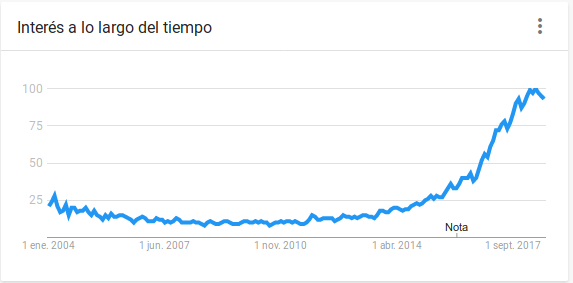
\includegraphics[scale=0.7]{./img/ml_google_trends.png} 
\end{center}

\begin{definicion}
\emph{Machine Learning}\\
Campo  de  estudio  que  da  a  los  ordenadores  la  habilidad  de  aprender  sin  la  
necesidad de ser explícitamente programados. 
Arthur Samuel, 1959
\end{definicion}

\subsection{Tipos de problemas en Machine Learning}
Hay tres tipos de problemas de machine learning: \textbf{Aprendizaje supervisado}, \textbf{Aprendizaje no supervisado} y \textbf{Aprendizaje por refuerzo}.  

\subsection{Aprendizaje Supervisado}
El objetivo principal del aprendizaje supervisado es construir un modelo a partir de un conjunto etiquetado de \textit{datos de entrenamiento} que nos permita hacer predicciones sobre los datos sin etiquetar que vengan en el futuro.  
Se llama aprendizaje supervisado porque la clave del paradigma radica en tener datos \textit{etiquetados} a priori.  
Hay dos tipos de problemas que se resuelven mediante aprendizaje supervisado:  
\textbf{Clasificación} y \textbf{Regresión}.

\subsection{Aprendizaje No Supervisado}
En el aprendizaje supervisado conocemos la \textit{respuesta correcta} de antemano cuando entrenamos nuestro modelo. En el aprendizaje no supervisado, por contra, estamos tratando con datos sin etiquetar o con datos con \textit{estructura desconocida}. Usando aprendizaje no supervisado podemos explorar la estructura de nuestros datos y extraer información util observando únicamente similitudes y diferencias entre los datos para poder agruparlos de forma que salgan a relucir posibles patrones ocultos en los datos.  
La técnica más popular dentro del aprendizaje no supervisado es el \textit{clustering}.
Este método se utiliza cuando se necesita clasificar las instancias de datos pero no se conocen previamente las categorías. Esta agrupación permite construir grupos (\textit{cluster}) de forma automática para clasificar de una forma lógica aun sin conocer las clases de antemano. 

Un ejemplo clásico es examinar los datos de ventas de una compañía para obtener grupos de clientes similares.


\subsection{Aprendizaje por refuerzo}
En el aprendizaje por refuerzo, el objetivo consiste en desarrollar un sistema (\textit{un agente}) que mejore su rendimiento basandose en interacciones con el entorno. Como la forma de aprender del entorno consite en la nueva incorporación de datos acompalañados de una medida de la \textit{función de recompensa}. Podemos pensar en el aprendizaje por refuerzo como un tipo de aprendizaje supervisado. Sin embargo en el aprendizaje por refuerzo esta etiqueta que acompaña a los nuevos datos no es una clase, como ocurre en el aprendizaje supervisado, sino que es una medida de como de bien o mal se está comportando el agente (valor de la función de recompensa asociado a los nuevos datos).  A traves de la interacción con el entorno un agente puede utilizar aprendizaje por refuerzo para aprender una serie de acciones que maximizen su recompensa mediante ensayo-error o mediante un plan deliberado.  

Un ejemplo clásico de aprendizaje por refuerzo es un programa que juegue a algún juego como el ajedrez. En este caso, el agente decide la jugada basandose en el estado actual del tablero (entorno) y la recompensa puede determinarse como una función que evalua cada situación y que lógicamente asigna la máxima puntuación a ganar y la mínima a perder.


\section{Resolviendo problemas con Aprendizaje Supervisado}
\subsection{Método de Regresión}
Este  método  se  utiliza  para  predecir  el  valor  de  un  atributo  continuo.  Consiste  en encontrar la mejor ecuación que atraviese de forma óptima un conjunto de puntos (n-dimensiones).  
Esta mejor ecuación se va a buscar dentro de una familia de funciones, de esta forma hablaremos de \textit{Regresión Lineal}, \textit{Regresión Logistica} etc...  
En estos métodos lo único que cambiamos es la familia de funciones, aunque también se pueden añadir mecanismos de regularización.


Supongamos que tenemos dos variables aleatorias $X$ e $Y$:
\begin{center}
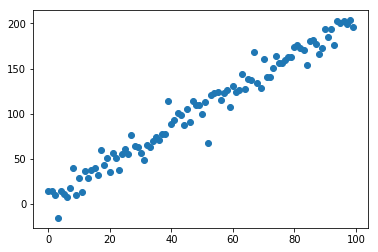
\includegraphics[scale=0.7]{./img/reg_lin_data.png}
\end{center}
Queremos buscar la mejor función lineal que exprese $Y$ como función de $X$:  
Aplicando regresión lineal obtenemos una función lineal $LM(x) = w_0 + w_1x$ tal que $LM(x) \simeq  Y(X)$ 
\begin{center}
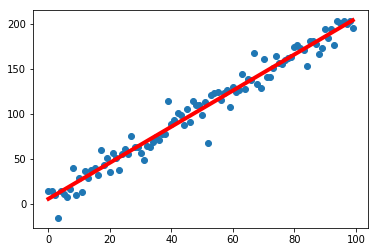
\includegraphics[scale=0.7]{./img/reg_lin_fit.png}
\end{center}

De esta forma ahora podríamos predecir el valor de nuevos datos colocandolos sobre la línea roja en la posición que les corresponda.  
Es decir: $y_{pred} = LM(X_{new})$

\subsection{Método de Clasificación}

Este método se utiliza para predecir a que clase pertenece una determinada instancia a partir de unas caraterísticas determinadas.  
El tipo más simple de clasificación es la clasificación binaria mediante un clasificador lineal:

Ejemplo: 
Supongamos que tenemos datos pertenecientes a dos clases (la clase violeta y la clase amarilla):
\begin{center}
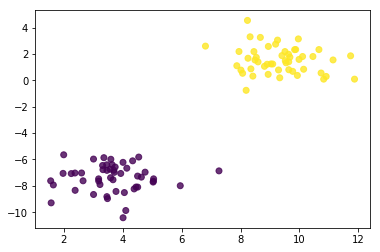
\includegraphics[scale=0.7]{./img/class_lin_data.png}
\end{center}
Queremos buscar la mejor función lineal que separe ambas clases:
\begin{center}
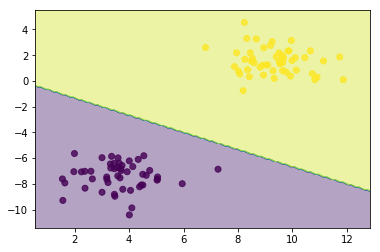
\includegraphics[scale=0.7]{./img/class_lin_fit.png}
\end{center}

\pagebreak

\subsection{Iris: El problema de clasificación más clásico}

En 1936 Ronlad Fisher anotó la colección de datos \textit{Iris}, en el que cuantificó varias mediciones taxonómicas de las flores de tres especies de Iris:

\begin{figure*}[!h]
$\begin{array}{rl}
    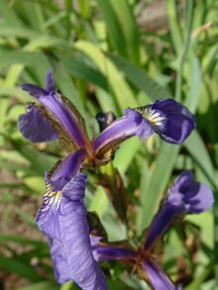
\includegraphics[scale=0.3, width=0.5\textwidth]{./img/Iris_setosa.png} &
    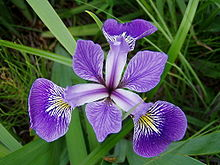
\includegraphics[width=0.5\textwidth]{./img/Iris_versicolor.jpg}\\
    \multicolumn{2}{c}{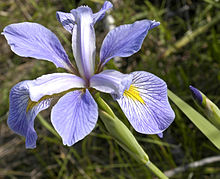
\includegraphics[width=0.5\textwidth]{./img/Iris_virginica.jpg}}
\end{array}$
\caption[Especies de Iris.]{\label{fig:label}Especies de Iris.}
\end{figure*}

\pagebreak
Podemos establecer como variables la longitud del sépalo y la longitud del pétalo y obtenemos una representación en 2D del conjunto de Fisher:

\begin{center}
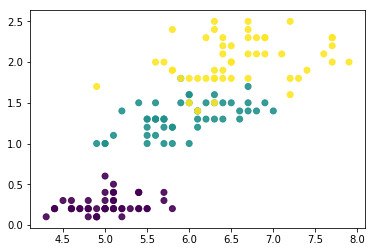
\includegraphics[scale=0.7]{./img/fisher_data.png}
\end{center}

Y podemos establecer muchos tipos de clasificadores:

El clasificador lineal que utilizamos antes se vería de este modo:

\begin{center}
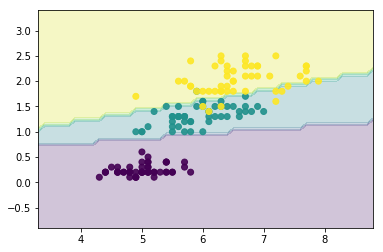
\includegraphics[scale=0.7]{./img/fisher_lin.png}
\end{center}

Pero podemos utilizar tambien clasificadores de tipo Boosting, concretamente el Gradient Boosting Machine, del que hablaremos más adelante y que ocupará la mayor parte del trabajo:

\begin{center}
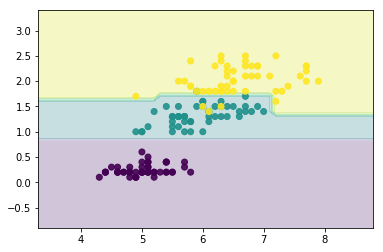
\includegraphics[scale=0.7]{./img/fisher_gbm.png}
\end{center}




\section{El flujo de trabajo para clasificación}

Todos los problemas de clasificación parten de un conjunto de datos etiquetados. Y el objetivo es construir una función que acepta nuevos datos con la misma estructura que en el conjunto inicial, pero sin etiqueta, y devuelve la etiqueta que considera que debe ser la correcta.  

Lo primero, antes de nada es separar el dataset en datos de entrenaminento (training dataset) y en datos de test (test dataset).  
Los datos de test se guardarán hasta el final sin hacer nada sobre ellos y se trabajará únicamente con los datos de entrenamiento.  
Para construir un modelo de calidad, primero deben \textbf{preprocesarse} los datos de entrenamiento, es decir, normalizarlos, escalarlos, aplicar transformaciones, seleccionar qué variables son importantes y cuales no...
Este es un subcampo bastante amplio llamado \textit{Ingeniería de Características}.  
Normalmente el preprocesamiento es la parte que más tiempo requiere y a la que el cientifico de datos más esfuerzo debe dedicarle.

Una vez se han preprocesado los datos de entrenamiento se utilizarán para \textbf{ajustar un modelo}, es decir, se construirá un modelo mediante un algoritmo de aprendizaje.

Una vez el modelo se ha construido llega el turno de \textbf{evaluar la calidad del modelo}, lo mejor es utilizar cross validation con los datos de entrenamiento para evaluarlo y dejar los de test únicamente para evaluar los modelos que creemos que son buenos.  
Existen técnicas para ajustar los parámetros empíricamente como por ejemplo \textit{gridsearch}.

Una vez tenemos un modelo de calidad podrá utilizarse para \textbf{predecir nuevos datos} y nuestro trabajo volverá a empezar para mejorar el modelo si así lo consideramos necesario.  

\begin{center}
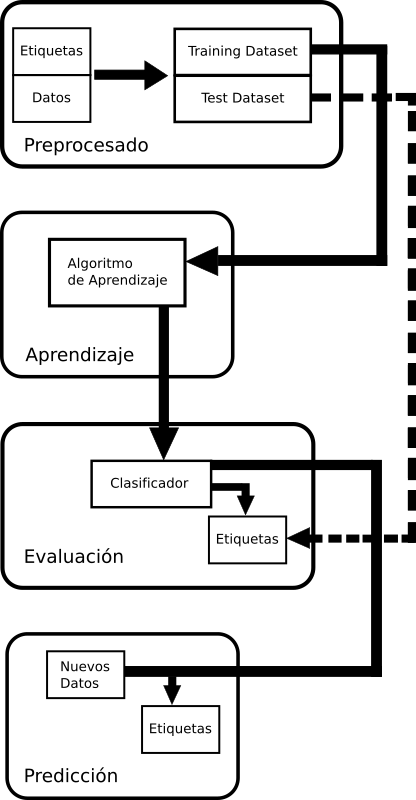
\includegraphics[scale=0.7]{./img/workflow.png}
\end{center}

\pagebreak

\section{Uso de Python para Machine Learning}
En este caso vamos a utilizar Python, debido a que actualmente se está convirtiendo en el lenguaje más utilizado para ciencia de datos, además de estar ganando terreno a muchos otros lenguajes clásicos debido a la enorme cantidad de librerías que existen para Python.  
La mayor alternativa a Python es el lenguaje estadístico R.  
No obstante un cientifico de datos debería conocer ambos lenguajes ya que R es muy potente a la hora de hacer un buen análisis exploratorio de forma rápida y eficaz.  
En Python también es posible trabajar como con R de forma rápida e interactiva utilizando Jupyter Notebook.  

Para lo que nos ocupa nos centraremos en utilizar las principales liberías de Python para Machine Learning:  

\begin{itemize} 
	\item{\textit{numpy}: Es una libería de cálculo numérico para Python, se encarga de que las opereciones computacionalmente intensivas con matrices se hagan con rutinas C muy eficientes en lugar de directamente interpretadas con Python}
	\item{\textit{pandas}: Es una libería para importar y exportar datos en Python, además con pandas es muy facil manejar grandes tablas de forma cómoda ya que está construida sobre \textit{numpy}} 
	\item{\textit{scipy}: Es otra colección de rutinas en Fortran y C para agilizar los cálculos científicos} 
	\item{\textit{scikit-learn}: Está contruida sobre \textit{numpy} y \textit{scipy} y tiene una gran cantidad de herramientas para poder completar el flujo de trabajo de un problema de machine learning sin necesidad de otras librerías en la mayoría de los casos sencillos} 
	\item{\textit{xgboost}: Es una librería que contiene la implementación del algoritmo XGBoost, el algoritmo de boosting más utilizado en la actualidad} 
	\item{\textit{matplotlib}: Es una librería para visualización de gráficos} 
\end{itemize}

\subsection{Instalación de Python y de paquetes}
Python está disponible para los tres grandes sistemas operativos (Linux, Microsoft Windows y Mac OS X).  
En la mayoría de distribuciones Linux modernas Python viene instalado por defecto en su versión moderna (Python3).  
En Mac no obstante aún viene por defecto la versión 2.7 (Python antiguo).
Lo ideal en este caso es instalar Python3 con un alias (python3) y utilizarlo, pero sin desinstalar el Python del sistema, ya que el sistema operativo utiliza internamente la versión 2.7 para algunas tareas.  
En Windows Python no viene instalado por defecto en ninguna versión por lo que hay que descargarlo de la web oficial: https://www.python.org  

Todo el código que se ha utilizado en este proyecto está escrito para Python3 y debería funcionar en todas las versiones superiores a la 2.7.10  

Para instalar paquetes en Python utilizaremos su gestor de paquetes \textit{pip}.

\begin{lstlisting}
pip install nombre_paquete
\end{lstlisting}

En nuestro caso vamos a instalar los paquetes básicos para probar el flujo de trabajo en machine learning.  
Más adelante profundizaremos en la utilización de los algoritmos de boosting.  

\pagebreak


% Insertar aqui Jupyter notebook ( Machine Learning basic workflow )

% \pagebreak


\section{Algoritmos de Boosting}

El boosting es un tipo particular de ensemble, consiste en un conglomerado de  clasificadores débiles (que son solo un poco mejor que la asignación aleatoria) que actúan de forma conjunta para construir un clasificador fuerte (de gran calidad). Un ejemplo típico de clasificado débil es un arbol de una sola hoja.  
En boosting se va construyendo el clasificador de forma iterativa, como ya mencionamos en la sección matemática.  
Las instancias que no han sido bien clasificadas en la iteración anterior adquieren una mayor importancia para la siguiente iteración. Podríamos decir que el algoritmo de boosting va concentrandose en acertar las instancias más dificiles conforme avanza en su proceso iterativo.  

Este proceso iterativo se ve reflejado en la siguiente ilustración:
\begin{center}
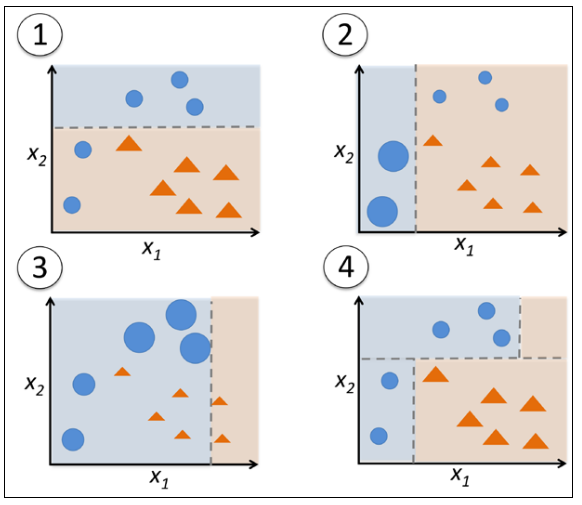
\includegraphics[scale=0.7]{./img/adaboost.png}
\end{center}

\subsection{Adaboost}

Adaboost es el algoritmo de boosting más simple.  
En Python puede implementarse definiendo un clasificador débil que actúe como base y construyendo el clasificador adaboost en base a él.  

A continuación podemos observar el mismo ejemplo del cáncer de mama aplicando Adaboost con árboles de una sola hoja como hemos explicado anteriormente.

\subsection{Extreme Gradient Boosting - XGBoost}
Adaboost es una forma de boosting simple pero poco eficaz en ejemplos reales.  
En la actualidad el algoritmo de boosting más famoso es XGBoost, una implementación muy eficiente del Gradient Boosting que aprovecha al máximo los recursos hardware disponibles.  

A continuación ilustramos el uso de XGBoost en el ejemplo anterior:

\section{Ruido de clase, Regularización, Underfing y Overfiting}



\section{Regularización en XGBoost}


















































\chapter{Conclusiones}




%
%
%
%%\nocite{*}
%\bibliography{bibliografia/bibliografia}\addcontentsline{toc}{chapter}{Bibliografía}
%\bibliographystyle{miunsrturl}
%
%\appendix
%\input{apendices/manual_usuario/manual_usuario}
%%\input{apendices/paper/paper}
%\input{glosario/entradas_glosario}
% \addcontentsline{toc}{chapter}{Glosario}
% \printglossary
\chapter*{}
\thispagestyle{empty}

\end{document}
